% New direct MC / LDA / MF comparison; numbers come from matched bulk runs.
% Generated from concentration-matched comparison.json
\newcommand{\MCScftZeroMC}{$58.561$}
\newcommand{\MCScftZeroLDA}{$50.911$}
\newcommand{\MCScftZeroMF}{$59.602$}
\newcommand{\MCScftBathShift}{$0.053$}
\newcommand{\MCScftMaxMfHeightDifference}{$2.607$}
\newcommand{\MCScftHeightRows}{%
$1$ & $54.63\pm0.26$ & $46.34$ & $54.83$ \\
$2$ & $46.02\pm0.21$ & $29.38$ & $46.94$ \\
$3$ & $39.28\pm0.35$ & $14.12$ & $40.37$ \\
}
\newcommand{\MCScftChargeRows}{%
$\overline\Gamma_{0.5}$ & $0.310\pm0.004$ & $-0.397$ & $0.324$ \\
$\Psi_{\rm rel}$ & $-0.599\pm0.244$ & $0.784$ & $-0.860$ \\
}

\pagetitle{Sampling versus PRL-type SCFT}{mcscftheight}
\smallnote{Matched physical parameters and measured bulk concentrations\quad /\quad 2026-09-07}
\textbf{Result: the 1D samples are closer to mean-field SCFT with correlations disabled.}
Blue denotes actual MC samples; red denotes the existing PRL-type smoothed-LDA SCFT;
green denotes SCFT with correlation self-energies disabled, retaining the mean potential and canonical C.
Black squares are digitized paper theory curves, distinct from our LDA implementation.

\begin{center}
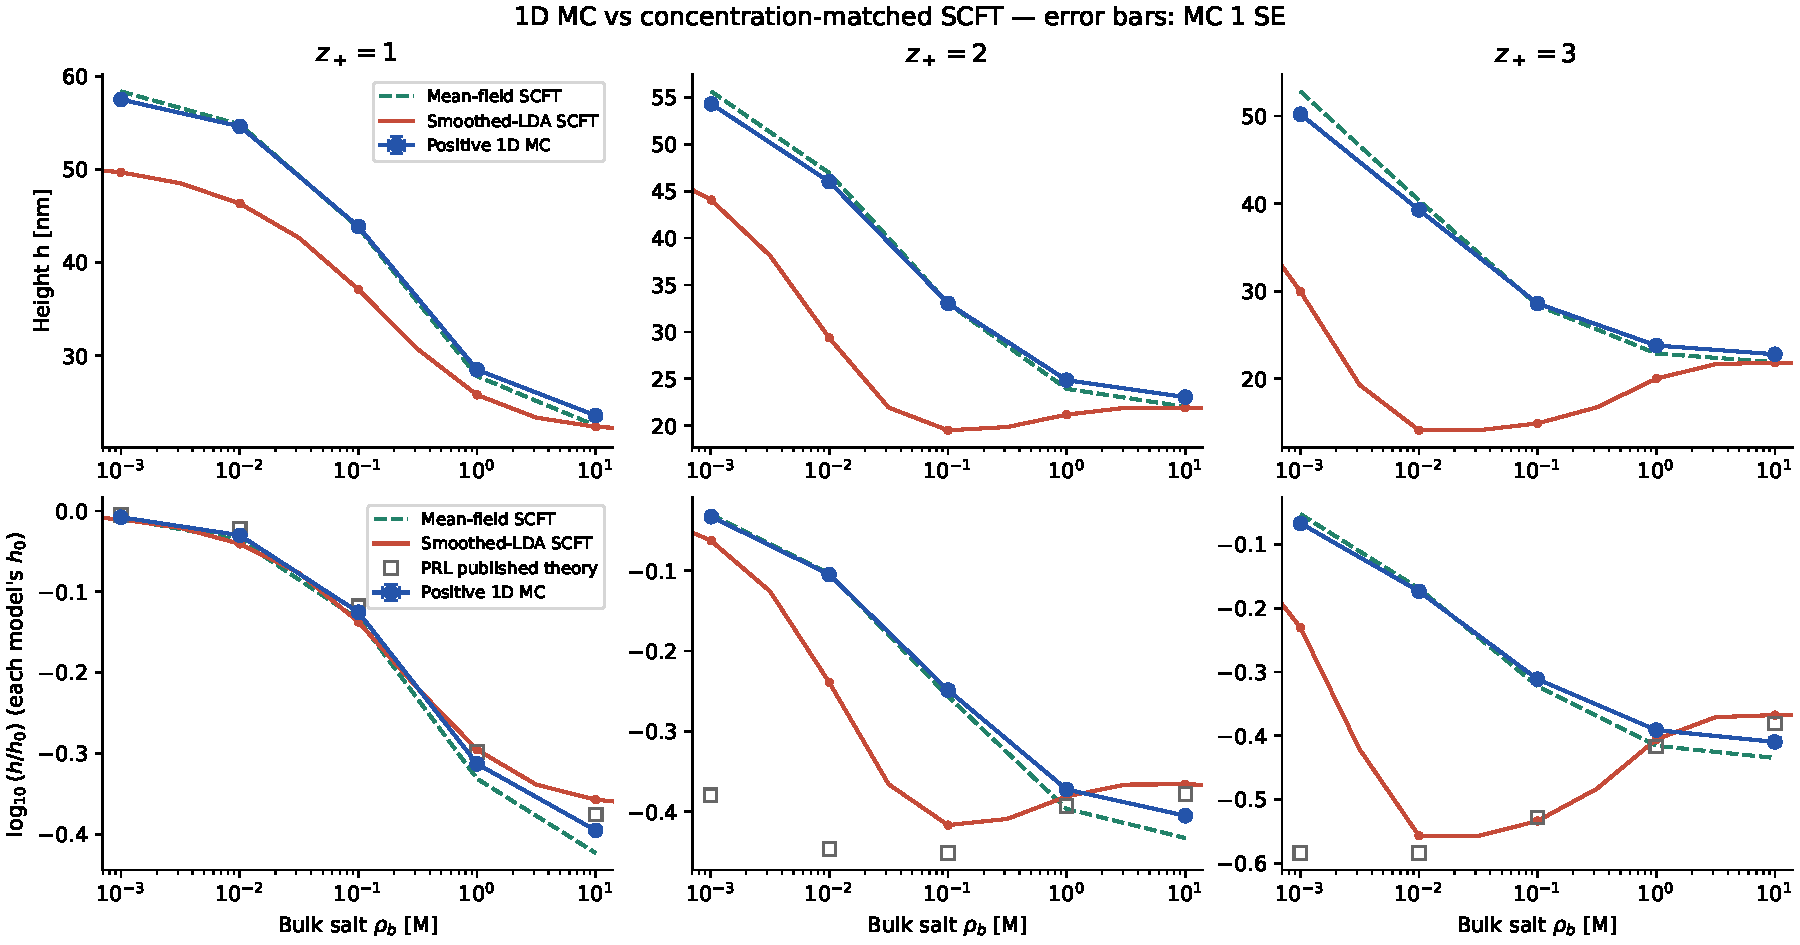
\includegraphics[width=\linewidth]{prl_comparison_figs/sampling_scft_20260907/mc_scft_height.pdf}
\end{center}
\vspace{-6pt}
\smallnote{Top: absolute height $h=2\int z\rho_P\,dz/(\sigma N)$.
Bottom: $\log_{10}(h/h_0)$, using each model's independently computed salt-free height.
MC error bars are 1 SE; the shared $h_0$ uncertainty correlates the normalized points.
Red lines show the earlier 19-point scan; small red dots are new solutions at the MC concentrations.}

\subhead{Heights near 0.01 M [nm]}
SCFT uses the actual MC bath concentration for each valence.

\begin{tabularx}{\linewidth}{@{}Xrrr@{}}
\toprule
\rowcolor{panel}$z_+$ & MC $\pm$ SE & LDA SCFT & Mean-field SCFT \\
\midrule
\MCScftHeightRows
\bottomrule
\end{tabularx}

Salt-free heights are MC \MCScftZeroMC\,nm, LDA \MCScftZeroLDA\,nm,
and mean field \MCScftZeroMF\,nm. These reference heights were not fitted to one another.
MC and mean field do not coincide: the largest absolute MC--MF height difference across
all comparison points is \MCScftMaxMfHeightDifference\,nm; some differences exceed the MC statistical errors.

\smallnote{$N=100$, $b=1\units{nm}$, $v=1\units{nm^3}$, $\sigma=0.1\units{nm^{-2}}$,
$\chi=0.5$, $\ell_B=0.7\units{nm}$, $a=0.25\units{nm}$, and $L=200\units{nm}$ were retained.
Replacing the nominal concentration with the measured MC bath concentration changes LDA heights by at most
\MCScftBathShift\,nm, insufficient to explain the large observed differences.
The paper uses a Gibbs dividing surface, so the normalized plot also compares different height definitions.}

\clearpage
\pagetitle{Charge, potential, and model differences}{mcscftcharge}
\begin{center}
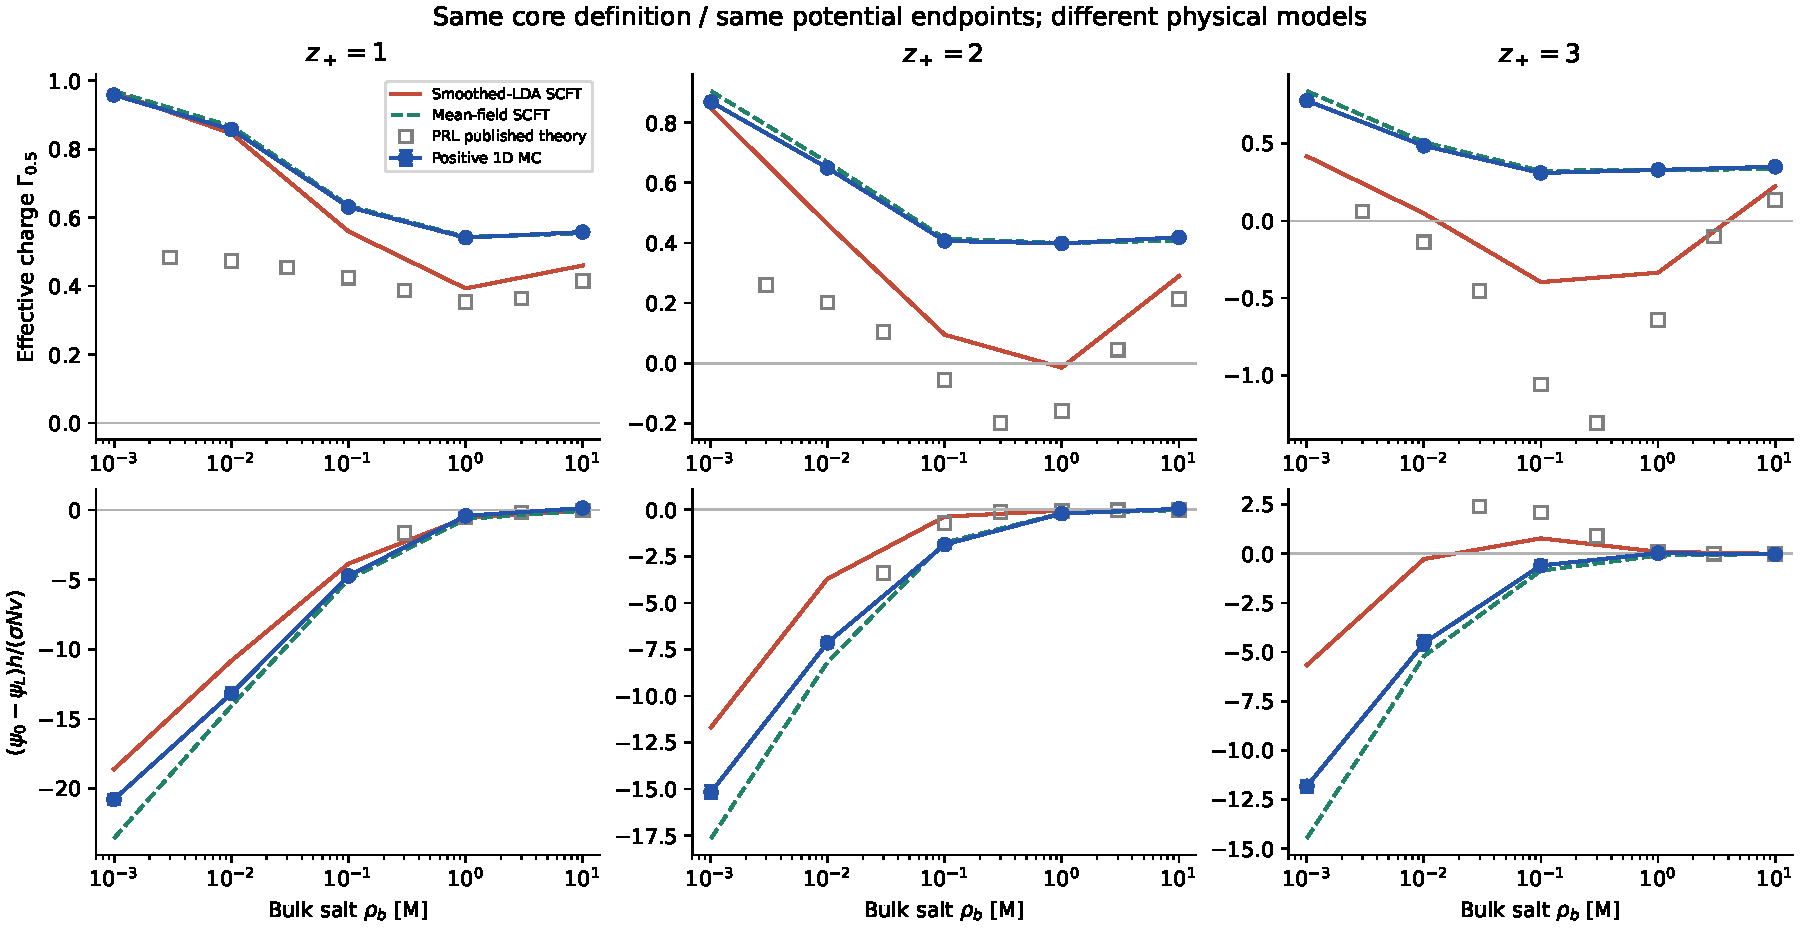
\includegraphics[width=\linewidth]{prl_comparison_figs/sampling_scft_20260907/mc_scft_charge.pdf}
\end{center}
\vspace{-7pt}
\smallnote{$\overline\Gamma_{0.5}$ is the salt-excess ratio in the core above half the polymer peak density.
SCFT densities were averaged over four cells onto the MC grid; potentials were compared at $z=0.25$, $199.75\units{nm}$.
This avoids mistaking an absolute gauge difference for potential reversal. Colors and symbols are as above.}

\subhead{Trivalent salt near 0.1 M: different charge and potential signs}
\begin{tabularx}{\linewidth}{@{}Xrrr@{}}
\toprule
\rowcolor{panel}Observable & MC $\pm$ SE & LDA SCFT & Mean-field SCFT \\
\midrule
\MCScftChargeRows
\bottomrule
\end{tabularx}

\subhead{A 1D mean profile can retain 3D fluctuations}
The PRL correlation theory includes a 3D charge Green function $G(\mathbf r,\mathbf r')$.
It retains transverse modes even for a planar mean density $\rho(z)$.
Its planar Fourier representation is
\begin{equation*}
 G(\mathbf r,\mathbf r')=
 \int\frac{d^2q_\parallel}{(2\pi)^2}
 e^{i\mathbf q_\parallel\cdot(\mathbf r_\parallel-\mathbf r'_\parallel)}
 G_{q_\parallel}(z,z')
\end{equation*}
The current MC samples a planar Coulomb action with only $q_\parallel=0$, excluding transverse fluctuations.
Increasing the sample count cannot restore those excluded correlation modes.
Our LDA approximates local 3D ionic correlations; equivalence to the paper's full nonlocal theory remains unverified.

This is a \textbf{comparison of different models}, not a test of MC algorithms for one action.
MC and MF also differ in finite $A$, integer cell solvent entropy, grid, charge smearing, and 1D fluctuations.
The PRL neglects $u_P^{\rm ex}$ but retains $u_P^0$; that omission alone cannot explain the discrepancy.
\smallnote{Theory: \href{https://arxiv.org/html/2404.09103v3}{Duan et al., Eqs.~(3)--(5)} and
SI Sec.~II. All new SCFT states passed full residual $10^{-7}$ and independent chain density/contour $Q$ checks at $10^{-10}$.
Numbers, density profiles, and run paths: \texttt{SAMPLING\_SCFT\_COMPARISON.md}.
The SCFT runs used the existing research runner; production FFT/C++/CUDA and MC/CL code were unchanged.}
